%
% Szakdolgozatminta az Eszterházy Károly Katolikus Egyetem
% matematika illetve informatika szakos hallgatóinak.
%

\documentclass[
% opciók nélkül: egyoldalas nyomtatás, elektronikus verzió
% twoside,     % kétoldalas nyomtatás
% tocnopagenum,% oldalszámozás a tartalomjegyzék után kezdődik
]{thesis-ekf}
\usepackage[T1]{fontenc}
\PassOptionsToPackage{defaults=hu-min}{magyar.ldf}
\usepackage[magyar]{babel}
\usepackage{mathtools,amssymb,amsthm,pdfpages}
\footnotestyle{rule=fourth}

\newtheorem{tetel}{Tétel}[chapter]
\theoremstyle{definition}
\newtheorem{definicio}[tetel]{Definíció}
\theoremstyle{remark}
\newtheorem{megjegyzes}[tetel]{Megjegyzés}

\begin{document}
\institute{Matematikai és Informatikai Intézet}
\title{Határidő napló webes és androidos platformon}
\author{Kertész Zoltán\\Programtervező informatikus BSc}
\supervisor{Dr. Tajti Tibor Gábor\\adjuntus}
\city{Eger}
\date{2022}
\maketitle
\tableofcontents

\chapter*{Bevezetés}
\addcontentsline{toc}{chapter}{Bevezetés}
A tanulmányaim alatt lehetőségem volt többféle programozási nyelv megismerésére. A szerver és a kliens oldali programozási nyelvek között is találtam olyat, ami elnyerte a tetszésemet. 

A mobil applikáció fejlesztéssel először egy beadandó feladatban találkoztam, majd később az ehhez tartozó órákat is elvégeztem, hogy elmélyítsem a tudásomat. A Java programozási nyelv elsajátítása nem okozott nagy kihívást köszönhetően a tanáraimnak. 

A webprogramozási ismeretek megléte úgy gondolom, hogy manapság alapvető elvárás, az itt töltött éveim során több erre szolgáló programozási nyelvel is megismerkedtem, számomra a PHP~\cite{php_doc} (PHP:Hypertext Preprocessor) vált a legkedveltebb programozási nyelvé. A számos PHP alapú keretrendszerek közül számomra a Laravel~\cite{laravel_main} volt ideális, alkalmas a terv megvalósítására, valamint az eddigi tanulmányok során áttfogó tudásra tettem szert vele kapcsolatban.

Ezért az lett a célom, hogy szakdolgozatomban ezeket a technológiákat használjam. Ezek felhasználásra rengeteg terv volt a fejemben, mire kialakult a jelenlegi projekt.

Véleményem szerint az emberek manapság inkább különböző applikációkat használnak, hogy a teendőiket nyilvántartsák, mint a hagyományos papír alapú noteszt. Viszont csak a mobilon tárolni a fontos feljegyzéseinket veszélyes, mivel az egy sérülékeny eszköz. A dolgozatom lényege, hogy egy olyan alkalmazást hozzak létre, amiben a felhasználók el tudják tárolni az eseményeiket és el is érjék azokat távolról is, platform függetlenül. Mivel az okos telefonok rendelkeznek beépített böngészővel így elég lenne, a probléma megoldásához csak a webes alkalmazás is, de szívesebben használják a felhasználók a kliens programokat. 

\chapter{Az alkalmazás bemutatása}
A szakdolgozatom projektje két részből tevődik össze. Az első rész egy webes alkalmazás a második pedig egy mobil applikáció. A fő összetevője a webes felület, mivel Androidon a projekt nem minden funkciója érhető el. 

A webes és az androidos alkalmazás tekintetében is törekedtem egy minimalista, mégis modern dizájn kialakításra, ami illeszkedik a világos és sötét témához is.
\section{Webes alkalmazás}
A projekt fő eleme a böngészőből elérhető alkalmazás. Itt került kialakításra a regisztráció és egy rövid ismertető a programról, hogy milyen feladatok, problémák megoldására terveztem. Ezek az oldalak elérhetőek a látogatók számára regisztráció nélkül. 

A felhasználónak regisztrációkor meg kell adnia a nevét, email címét és jelszavát. Ha a regisztráció sikeres egy levelet küld ki az alkalmazás a megadott címre ahol a regisztrációkor kitöltött név jelenik meg és egy gomb ami átirányítja a felhasználót a webes felületre. Bejelentkezés után a felhasználó korlátozás nélkül tudja használni az alkalmazás nyújtotta lehetőségeket. 

A navigációs részben a legördülő menüben az események alatt lehetőség van új esemény hozzáadására, a meglévők kilistázására annak megfelelően, hogy melyik csoportba tartozókat szeretnénk megjeleníteni. Ilyen kategóriák az aktív, teljesített és lejárt események. 

Ahhoz, hogy a használó új eseményt tudjon hozzáadni kötelező annak nevet, kezdési és befejezési dátumot adni. Mentés közben ezeken az adatokon ellenőrzés fut le, hogy a kitöltés a szabályoknak megfelelő legyen. Ilyen előírás, hogy a név és dátumok ki legyenek töltve. A dátumokra másik szabály is vonatkozik, mégpedig, hogy a kezdési időpont ne lehessen korábban, mint az aktuális dátum és a befejezési idő nem lehet korábban, mint a kezdési. Ha ezeknek a bevitt értékek megfelelnek akkor megtörténik az eseménynek a mentése és közben az alkalmazás levélben értesíti a felhasználót, amiben leírja neki az eseményhez tartozó elnevezést, leírást, kezdési és befejezési dátumot. 

Az feljegyzések közötti kilistázás első eleme az ,,Aktív események''. Az alkalmazásomban az számít futónak, ahol a befejezési időpont nem korábbi, mint az éppen aktuális dátum és az adatbázisban a ,,complete''  attribútumban 0 szerepel.

A menüben a következő választható lehetőség a ,,Lejárt események'' listája. Itt van lehetősége a felhasználónak megtekintenie azokat az eseményeket amiket nem teljesített, de már nem is aktívak. Lejárt eseménynek a rendszerben az számít ahol a befejezési dátum korábbi, mint az aktuális dátum és a ,,complete'' oszlop értéke szintén 0. 

A fenti két eseményben az a közös, hogy a kliensnek lehetőse van a módosításra, teljesítésre és a törlésre is. Módosításkor a hozzáadási szabályok érvényesek az adatokra.

A legördülő menü utolsó eleme pedig a ,,Teljesített események''. Itt lehet megtalálni azokat az eseményeket ahol a ,,complete'' oszlopnak 1 az értéke. A megjelenő rekordok a módosítási dátumuk alapján csökkenő sorrendben kerülnek megjelenítésre. A teljesített események fontos különbsége, hogy a módosításra már nincsen lehetősége a felhasználónak, csak a törlésre.

A következő választható menü elem a ,,Profil''. Itt egy olyan oldal jelenik meg, ahol a bejelentkezett felhasználó adati kerülnek kiíratásra. Az információk alatt egy legördülő menü található amiben a profilon elvégezhető műveleteket érhetjük el.

A ,,Profil módosítás''-t választva megjelennek a felhasználó adatai. Amennyiben egy adatot nem szeretnénk módosítani úgy azt nem kell átírni. A mentésre kattintva az adatokat ellenőrízük,  ahol a következő szabályoknak meg kell felelni: a név mező nem lehet üres, az e-mail cím nem lehet üres és tartalmaznia kell ,,@'' írásjelet.

Lehetőség van jelszó módosításra is, amit a következő menüpont biztosít. Jelszó módosításkor egyértelmű, hogy az üres mezők esetén hibával térünk vissza. Ezen kívül az új jelszót kétszer kell megadni és vizsgáljuk, hogy ugyan azok-e a jelszavak. Ezt követően az új jelszónak beírt karakterláncot kódolva eltároljuk, kijelentkeztetésre kerül a felhasználó és át lesz irányítva a bejelentkező oldalra, ahol már az új jelszóval kell bejelentkeznie.

Az utolsó funkció amit a felhasználó elér ebben a menüben az a profiljának a törlése. Hogy ez sikeres legyen meg kell adni kétszer a jelenlegi jelszót. Ha a törlés sikeres a felhasználó az applikáció főoldalára lesz irányítva, amennyiben sikertelen egy hiba üzenettel küldjük vissza a törlési oldalra.

A navigációs fül utolsó lehetőse a ,,Kijelentkezés''. A bejelentkezett felhasználó itt ki tud lépni az alkalmazásból és a kezdőoldalra kerül. 

\section{Androidos alkalmazás}
A kliens program Androidos telefonokra készült alkalmazás ami API~\cite{api_basic} kapcsolaton keresztül kommunikál a webes szoftverrel. Az alkalmazás nem tárol lokálisan adatot, ezzel került megoldásra az a probléma, hogy esetleges meghibásodás esetén adat vesztés történne. 

Az alkalmazás első megnyitása után egy bejelentkezési felület fogadja a felhasználót ahol meg kell adni az e-mail címét és jelszavát. Ezen két adat ellenőrzése két helyen valósul meg. Először az alkalmazás megvizsgálja, hogy nem-e üresek a mezők, amennyiben nem írtunk bele adatot hibaüzenetet kapunk. Ha kivannak töltve a mezők egy REST kérést küldünk. Amennyiben a válasz nem a felhasználó adatai egy szöveg buborék jelenik meg, hogy hibás a bevitt adat, máskülönben sikeres a bejelentkezés és a kezdőképernyő jelenik meg.

A főoldalon lehetőség van új eseményt hozzáadni vagy kilistázni az aktív, lejárt vagy teljesített feljegyzéseket. Ezen kívül található még egy felugró menü ahol minden funkciót megtalálunk amit elérhetünk az alkalmazásban. A menüben olyan pontokat találhatunk ami az esemény hozzáadás, listázás típusonként, feljegyzés kezelése, profil szerkesztése és a kijelentkezés. 

Az esemény hozzáadása több helyről is elérhető, mivel ez egy alap funkció, ezért kézközelben kell lennie. Amikor megnyílik a hozzáadásért felelős nézet a már webes felületen megszokott adatok bevitelére van lehetőség. Dátumot egy felugró ablak segítségével lehet beállítani, majd megjelenítjük a kiválasztott időpontot. 

A főoldalon a bejelentkezett felhasználót egy üdvözlő üzenet fogadja, ahol a regisztrációkor megadott név szerepel. Ezen kívül elérhetjük a hozzáadás funkciót és esemény csoportonként a listázást. 

A csoportonként megjelenítendő eseményeknél a felhasználó a következő adatokat látja: az esemény azonosítója, neve, leírása, kezdeti és befejezési dátum. A webes felülethez hasonlóan itt is kártyaként jelennek meg az adatok. 

Az ,,Esemény kezelése'' menüpontban van lehetőség módosítani, késznek jelölni és törölni az adott eseményt. Először a felhasználónak le kell ellenőriznie, hogy az esemény létezik-e, ehhez meg kell adnia az azonosítóját. Amennyiben nem létezik egy felugró szöveg buborék jelenik meg, hogy helytelen az azonosító. Ha sikeres volt az ellenőrzés megjelenik a kiválasztott azonosítóhoz tartozó adatok. Mentés esetén a már webes felületen ismertetett szabályok kerülnek ellenőrzésre. Amennyiben üresen hagyja a felhasználó a nevet vagy a dátumok közül valamelyiket egy hiba üzenet kerül kiírásra ahol megjelenítésre kerül, hogy mely adatokat kell leellenőrizni. 

A ,,Profil'' menüpontot választva megjelenik az aktuálisan bejelentkezett felhasználó adatai amit módosítani lehet. A sikeres módosítás után az alkalmazás egy szöveg buborékban tájékoztatja a felhasználót a sikerességről. 

A felhasználói adatokat bejelentkezés után megjegyzi a kliens program így nem kell minden megnyitáskor belépni csak, ha a menüben kijelentkezünk az alkalmazásból. 

\chapter{Fejlesztői környezet}
\section{Web szerver}
Az alkalmazások működéséhez szükséges egy web szerver. Ehhez több lehetőség is van a fejlesztők részére. Virtualizálhatunk egy Linux alapú szervert ahol kialakítjuk a LAMP~\cite{lamp_book} (Linux, Apache, PHP, Myadmin) környezetet. Létrehozhatjuk a programunkat Dockerben~\cite{docker_doc}, ami egy virtuális szervernek felel meg, vagy használhatunk olyan segéd programot, mint a XAMPP~\cite{xampp_doc} vagy a WAMPP~\cite{wamp_doc}. 

Személy szerint nekem sokkal jobban bevált a XAMPP, így dolgozatom fejlesztése alatt is azt használtam, mivel egyszerű a telepítése és a kezelhetősége. Mindemellett lehetőség van konfigurálni azt is, hogy milyen adatbázist szeretnénk használni. 

\section{Kód szerkesztő}
Ha már van környezetünk ahol majd a webes projektünk futtathatóvá válik keresnünk kell egy olyan szöveg szerkesztőt amit használni fogunk. Program fejlesztésre több ilyen eszköz is létezik, ami segíti a programozó munkáját szöveg kiemeléssel, kód kiegészítéssel és szintaxis ellenőrzéssel. Számomra a legjobban bevált ilyen program a ,,Visual Studio Code''~\cite{vsc_doc} ami ingyenes szövegszerkesztő és különböző bővítményekkel lehet kényelmesebbé tenni a használatát.

\section{Android alkalmazáshoz Adroid Studio}
Androidos alkalmazás fejlesztésére többféle eszköz áll a rendelkezésünkre. Ilyen lehetőség lehet az ,,Eclipse''~\cite{eclipse_doc} vagy esetleg a ,,RAD Studio''~\cite{rad_doc}. Számomra a leginkább preferált fejlesztői környezet az ,,Android Studio''~\cite{androidStudio_doc}. Azért tartom jobbnak a többinél, mivel nem csak mobil eszközre lehet vele alkalmazást írni, hanem Wear OS-es órára és TV-re is. A másik előny, hogy a felhasználói kezelő felület kialakításához biztosít egy tervezőt ahol az elemeket fogd és vidd (drag and drop) módszerrel lehet elhelyezni a megjelenítő felületre. 

Az ,,Android Studio''-ba olyan fontos funkciók vannak beépítve, mint az AVD~\cite{androidStudioAvd_doc} menedzser (manager), ami egy emulátor, ahol virtuális eszközöket tudunk létrehozni, hogy tesztelni tudjuk az alkalmazásunkat. A másik fontos eszköz ami implementálva van az ADB~\cite{androidStudioAdb_doc} (Android Debug Bridge) ami a virtuális vagy fizikai eszközünk között kommunikál a számítógéppel így figyelve az alkalmazásunk működését és hiba esetén megkönnyíti a hiba keresést. 
\section{Postman a REST API-hoz}
A REST API kapcsolat teszteléséhez szükség volt egy kliens programra, ahol lelehet ellenőrizni, hogy a kérés sikeres-e és a válasz megfelelő-e. Ehhez a ,,Postman''~\cite{postman_doc} programot választottam, mivel kliens program, egyszerű a használata ezért nem csak egy személy vehet részt a tesztelésben, mindezek mellett lehetőség van a teszteket kollekcióba elmenteni amiből későbbiekben automatizált teszt is futtatható. A szoftver nagyon sok API szabványt és formátumot támogat köztük a ,,JSON''-t~\cite{json_doc} is.

\chapter{Az alkalmazás felépítése}
\section{Miért PHP és Laravel?}
A szerver oldali programozási nyelvek között még mindig vezető helyen szerepel a PHP, köszönhetően annak, hogy széles körben használt, egyszerű és könnyen tanulható nyelv. A másik vezető nyelv a JavaScript~\cite{js_book} amit leginkább ,,SPA'' (Single Page Application / Egyoldalas alkalmazások) fejlesztésére használnak. 

Számomra a PHP azért lett kedvesebb, mivel széleskörűen használható, gyors, rugalmas és jól dokumentált. 

Mivel tisztán PHP kódot már kevés helyen használnak, leginkább kis projektek esetén így érdemes keresni egy keretrendszert. Nagyon sok lehetőség van az interneten amit használhatunk, de talán a legelterjedtebb ilyen a Laravel~\cite{laravel_book}. 

A Laravel több szempontból is ideális választás webes alkalmazásokhoz, mivel megkönnyíti az olyan általános feladatokat, mint az útvonalválasztás (routing) és a hitelesítés. A keretrendszer követi az MVC~\cite{mvc_pattern} (Model View Controller / Modell Nézet Vezérlő) tervezési mintát, ezért hatékonyabb, biztonságosabb és a projekt átlátható lesz. 

Szinte minden webes alkalmazás kommunikál valamilyen adatbázissal. A Laravel ezt a kommunikációt teszi egyszerűbbé a Query Builder~\cite{laravel_querybuilder} (lekérdezéskészítő) és az ORM (Object Relational Mapping / Objektum-relációs leképezés) használatával. 

\section{Sass és CSS}
A CSS~\cite{css_doc} állományok gondoskodnak a frontend dizájnjáról. Ez sajnos sok hiba lehetőséggel jár, mivel egyetlen nagy fájlban tároljuk a megjelenésre vonatkozó információkat. Ennek eredménye, hogy nagy projektben strukturálatlanná válik az állomány aminek rendszerezése igen nagy feladat lenne. Erre jó mód lenne külön állományban tárolni az egyes oldalakra vonatkozó CSS információkat, de ez több kérés lenne a szerver felé. 

Ennek a problémának a megoldására léteznek olyan előfeldolgozók (pre-processor), mint a Sass~\cite{sass_doc}, ahol lehetőség van több rész állományt létrehozni ezzel javítva a struktúrát. Az előfeldolgozó végül pedig egyetlen fájlba egyesíti a részeket és nem növeli a kérések számát. 

\section{Bootstrap}
A Bootstrap~\cite{bootstrap_doc} egy olyan nyílt forráskódú CSS keretrendszer ami megkönnyíti a frontend programozást az előre definiált komponensekkel. Ez a technológia minimális erőfeszítést igényel a fejlesztő részéről, hogy implementálja saját projektjében. Az előre definiált komponensek tartalmaznak HTML, JavaScript és CSS elemeket, melyeket a későbbiekben könnyű módosítani.

A webes alkalmazásom tervezését ezzel végeztem és a későbbiekben saját ízlésemnek megfelelően írtam felül a szükséges elemeket. 

\section{MariaDB, mint adatbázis}
A piacon nagyon sok SQL~\cite{sql_book} alapú relációsadatbázis-kezelő szoftver létezik, ezek egyike a MariaDB~\cite{mariadb_doc}, ami egy nyílt forráskódú többfelhasználós adatbázisszerver. A legismertebb szerverek közé tartozik a MySql~\cite{mysql_book} ami az Oracle tulajdona. A MariaDB és a MySql között nagyfokú a kompatibilitás, mivel a MariaDB a MySql-nek a nyílt forráskódú részeiből alakult ki. Másik fontos előny a kompatibilitás tekintetében, hogy egymást ki tudják váltani.

\section{Java}
Manapság az Androidos operációs rendszerre történő fejlesztéskor inkább a Kotlin~\cite{kotlin_book} nyelv van feltörekvőben, mivel a Google ezt támogatja, de nem elhanyagolható a Java programozási nyelv jelenléte sem, hiszen más területeken még mindig fontos szerepe van. 

Számomra a Java programozási nyelv a kedveltebb, mivel viszonylag független az operációs rendszertől és olyan könyvtárakat tartalmaz amik elősegítik a programozó munkáját. Mindezek mellett a Java idősebb nyelv, mint a Kotlin így sokkal több ismeret anyag érhető el hozzá.

\chapter{Webes alkalmazás}
\section{Migráció}
\subsection{Általános információk}
A migráció (migration)~\cite{laravel_migartion} segít az adatbázis tábláinak létrehozásában, továbbá, ha az adatbázisban valamilyen módosítást kell végrehajtani akkor ezen fájlok lefuttatásával újra tudjuk generálni a táblákat. Ahhoz, hogy új migrációt adjunk a projektünkhöz egy terminálra van szükségünk, ahol a projektünk mappájában tartózkodunk. Ekkor a következő parancsot kell lefuttatni: ,,php artisan make:migration tabla\_neve''.

A migráció létrehozásakor két metódust találunk: ,,up'' és ,,down''. Az ,,up'' metódus új táblák, oszlopok, indexek hozzáadására szolgál, míg a ,,down'' pedig a módosítások visszaállításra szolgál. 

\subsection{Migráció a felhasználóhoz}
Az felhasználóhoz tartozó tábla migrációjában kétféle adat szerepel: felhasználó által kitöltött, generált. A bevitt adatok közé tartozik a név, e-mail cím, jelszó. Az elektronikus levelezési címhez tartozik egy megkötés ami biztosítja, hogy egyedi (unique) minden felhasználónál. 

A generált adatok a következőek: id, remember\_token, created\_at, updated\_at. Az emlékezz token (remember token) akkor kerül kitöltésre, ha a felhasználó szeretné, hogy a weboldal megjegyezze a bejelentkezést és bejelentkezve tartsa. Ez a token akkor frissül, mikor a bejelentkezett kliens kijelentkezik. Ez egy biztonsági funkció, arra az esetre, ha eltérítenék a sütit (cookie), akkor egy egyszerű kijelentkezéssel érvénytelenítődjön. 

A created\_at és updated\_at egy dátum típusú mező ami szintén legenerálódik, amikor a felhasználó regisztrál vagy módosítja az adatait. 

Az id attribútum automatikusan növekvő szám sorozat amivel egy egyed beazonosítható, tehát ez az elsődleges kulcs az adattáblában.  A kulcs minden esetben előjel nélküli szám.
\subsection{Migráció az eseményhez}
Az eseményben is szerepelnek generált és felvitt adatok. A generáltról nem beszélnék, mivel nagyban megegyezik a felhasználó migrációban szerepelt generált adatokkal. A különbség az eseményre vonatkozó, felhasználó által beírt adatokban van. 

Generálódó adatok közül amit érdemes megemlíteni az esemény táblánál a user\_id, ami egy külső kulcs. Itt az aktuálisan bejelentkezett felhasználó id-ja kerül eltárolásra. 

A felhasználónak a következő mezők kitöltésére van lehetősége: topci, description, start, end és complete. 

A topic az esemény neve, ahol karakterláncot (string) tárolunk el, amelynek maximális mérete 255 bájt lehet. A következő az esemény leírása. Ez egy text formátumú attribútum, melynek a maximális mérete 65.535 karakter hosszúságú.

Az kezdési és befejezési dátumnál események távozása révén fontos kritérium volt, hogy nem csak dátumot, hanem időt is tárolni kell. Erre a legjobb megoldás a datetime típus ahol a legnagyobb megadható dátum a ,,9999-12-31 23:59:59''.

\section{Modellek}
A modellek a MVC~\cite{mvc_mozzilla} tervezési mintában az adatbázis és a vezérlő közötti kapcsolat. Itt definiálhatjuk az adatok láthatósági szintjét és, hogy az adott szinten mik érhetőek el.
\subsection{Felhasználói modell}
A modell definiálása a kitölthető adatokkal kezdődik, melyek jelen esetben a név, e-mail és jelszó. A következő attribútumokat a rejtettek. Ezek a jelszó és a tokenek. Majd a végén található egy olyan metódus ami a kapcsolatot képezi a felhasználó és az esemény modell között. Itt jelen esetben azt adjuk meg, hogy egy felhasználóhoz több esemény is tartozhat.

\subsection{Esemény modell}
Az esemény lényegében sokkal egyszerűbb, mint a felhasználónak a modellje, mivel itt csak kitölthető mezőkkel találkozunk. Ezek a mezők a következők: topic, description, start és end.

\subsection{Eloquent ORM}
Ugyan ez nem modell, hanem az adatbázissal való kommunikációt biztosítja. Azért tartom fontosnak megemlíteni a modellek között, mivel ez teszi lehetővé az adatbázisba való rekord beszúrást, lekérdezést és törlést. Amennyiben az adatbázisunkban a tábla neve nem azonos a modellével akkor meg kell adni, hogy mi a tábla neve. Az eloquent orm~\cite{laravel_eloquent} és query builder előnyeiről a kontroller osztályban fogok még írni.

\section{Nézetek}
A nézetek (view) felelnek a megjelenítésért. Jelen projektben a nézeteket két csoportba osztanám, melyek a következők: felhasználói nézet és e-mailhez tartozó nézet. A Laravel a nézetekhez a Blade~\cite{laravel_blade} sablonozó motort használ, ami egyszerű és ugyan úgy lehet benne PHP kódot futtatni. A blade sablonok meghívhatóak útvonalról és vezérlőből is, ennek köszönhetően teljesül a MVC tervezési minta. 

A Blade sablonban lévő PHP kódunkat dupla kapcsos zárójelek közé kell tenni. Ilyen PHP kód lehet egy útvonal hívás vagy olyan adat megjelenítés ami a szervertől érkezik. Ezen kívül a Blade-ban lehetőség van az alapvető vezérlési szerkezetek implementálására, mint például az if, foreach.

\subsection{Felhasználói nézetek}

Egy felhasználói nézet két komponensből tevődik össze, egyik az úgynevezett keret és maga a tartalom. A keret tartalmazza a HTML~\cite{html_doc} fejlécet ami a következőket foglalja magába: milyen néven található a CSS állomány, az alkalmazás ikonja és a JavaScript meghívása. Ezen kívül itt szerepel még a navigációs menü és egy @yield kulcsszó ami egy szakasz tartalmának megjelenítésére szolgál. A navigációs menüben találhatunk egy felhasználó ellenőrzést, ugyan is látogató annak megfelelően láthatja a menü elemeket, hogy be van-e regisztrálva.

Mielőtt definiálnánk egy szakaszt meg kell adni, hogy melyik elrendezést örökölje, illetve esetemben, hogy milyen keretet örököljön erre a @extends kulcsszóval kell hivatkozni. A szakaszokat @section és @endsection segítségével definiáljuk.

Az egyes esemény csoportok megjelenítésénél az if vezérlési szerkezettel ellenőrzöm le, hogy milyen típusú eseményt kapok vissza. Ennek megfelelően lesz az események alatt a módosításhoz vagy törléshez szükséges interakció gombok. Ezen kívül az események megjelenítésénél találkozhatunk még foreach ciklussal ahol az egyes elemek és hozzájuk tartozó gombok külön kártyában jelenítődnek meg. 

\subsection{E-mailhez tartozó nézetek}
A kiküldött e-mailekhez tartozó nézetek külön vannak definiálva, mivel eltérnek a felhasználóitól, ugyan is, itt a Blade sablonozó motor komponenseit használjuk és a MarkDown~\cite{markdown_page} szintaxisát. Ennek köszönhetően az e-mailünkben nem csak szöveget tudunk küldeni, de gombot is, mely átirányíthat minket az alkalmazásra vagy a már meglévő útvonalak valamelyikére.

\section{Kontrollerek}
A kontrollerek~\cite{laravel_controller} dolgozzák fel a felhasználói műveleteket és válaszol azokra. A kontrollerekben gyűjtjük össze azokat az adatokat amik a felhasználói felületről érkeznek és ha kell meghívjuk a modellt, hogy tárolja el azokat az adatbázisban. Amennyiben az adatbázisból érkeznek az adatok úgy azt tovább küldjük a megjelenítéshez. Mivel dolgozatomban a felhasználó kétféle szerepkört tölthet be, miszerint lehet látogató vagy bejelentkezett felhasználó így ezt ellenőrizni kell, hogy a jogosultságának megfelelő oldalakat érje el. Ehhez definiálni kell egy konstruktort ahol a köztes szoftver (middleware)~\cite{laravel_middlewear} ellenőrzi, hogy a felhasználó be van-e jelentkezve vagy vendég.
A vezérlők általános működése a következőképpen írható le:~\cite{controller_cicle}
\begin{itemize}
\item{A felhasználó valamilyen interakciót létesít a kezelő felülettel.}
\item{A vezérlő átveszi a küldött adatokat a felhasználó felülettől.}
\item{Kapcsolat létesítése a modellel, és ha szükséges az adatok módosítása.}
\item{ A nézet a válasz alapján létrehozza a megfelelő kezelési felületet. A nézet a modellből nyeri az adatokat, de a modellnek nincs közvetlen tudomása a nézetről.}
\item{A felhasználói felület újabb interakcióra vár és kezdődik elölről a kör.}
\end{itemize}
\subsection{Regisztráció kontroller}
A regisztráció csak a látogatók (guest) számára elérhető oldal. Első lépésben ezt ellenőrizni kell, hogy a felhasználó be van-e jelentkezve. Ezt a köztes szoftver (middleware) ellenőrzi. Amennyiben bejelentkezett felhasználó hívná meg a regisztrációért felelős kontrollert a profilra kerül átirányításra. Ha ténylegesen a vendégtől érkezik a kérés akkor meghívódik a regisztrációhoz tartozó kontroller.  

Amikor meghívódik a következő adatokat vizsgáljuk ami a felhasználótól érkezik: név, e-mail cím, jelszó és az ,,aszf''.
Sorban haladva a névre vonatkozó szabályok aminek meg kell felelni a bevitt adatnak:kötelező kitölteni, maximum 255 hosszú lehet. A következő az e--mail cím ahol a névhez képest annyi kiegészítést tartalmaz, hogy elektronikus levelezési cím formátumnak kell lennie, tehát ,,@'' jelet kell tartalmaznia.
A jelszó is kötelező adat aminek minimum 6 karakterből kell állnia és meg kell erősíteni. Az utolsó az általános szerződési feltételekhez tartozó jelölőnégyzet (checkbox), amit be kell pipálni.

Ha a validáció sikeres a kontroller megvizsgálja, hogy a beírt e-mailcím már szerepel-e az adatbázisban. Itt elő is jön az eloquent és a query builder előnye, hogy nem kell kézzel lekérdezést írni, hanem egyszerűen meghívjuk a modellt és annak az ahol (where) metódusát. Itt megvizsgáljuk, hogy az e-mailcím szerepel-e már az adatbázisban. Ehhez a ,,count'' aggregátumot társítjuk ami megszámolja, hogy a lekérdezés mennyi sort adott vissza. Amennyiben szerepel, tehát a visszatérési érték 1, visszatérünk a nézetre ahol megjelenítjük, hogy hibás az cím, mert szerepel már az adatbázisban. Amennyiben az eredmény 0 eltároljuk az adatokat úgy, hogy az adatbázisban szereplő attribútumához a kérés tömb megegyező adatát társítjuk. Kivételt képez ez alól a jelszó ahol előtte meg kell hívnunk a Hash osztály készít (make) függvényét a kérésben szereplő jelszóra, hogy kódolva tároljuk el azt. Mentés után a felhasználót bejelentkeztetjük amiben segítségünkre lesz az Auth~\cite{laravel_auth} osztálynak az attempt metódusa ami megvizsgálja, hogy a kérésben kapott e-mail cím és jelszó páros szerepel-e az adatbázisban. A metódus visszatérési értéke lehet igaz vagy hamis, annak megfelelően, hogy sikerült-e megtalálni az beírt adatokat. Ezt követően egy e-mailt küld ki a rendszer a megadott levelezési címre amelyben köszönti a frissen regisztrált felhasználót. Végül pedig átirányítjuk a saját profil oldalára.

\subsection{Bejelentkezéshez használt kontroller}
A bejelentkezésért felelős kontroller meghívásakor is vizsgálni kell, hogy már be van-e jelentkezve a hívó fél. Ennek az ellenőrzéséért a kontrollerben szereplő konstruktorban lévő middlewear a felelős. Ha egy bejelentkezett felhasználó próbálja elérni a bejelentkezést a profiljára kerül átirányításra, amennyiben nincs bejelentkezve úgy elérni a vezérlőt.

A bejelentkezéskor lefut egy ellenőrzés a felhasználó által beírt adatokra ahol a következő szabályoknak kell megfelelni: az e-mail cím és jelszó nem lehet üres és az e-mail címben szerepelnie kell a ,,@'' karakternek.

Az Auth osztály itt is nagy segítségünkre van és elvégzi az adatvizsgálatot és bejelentkeztetést. Amennyiben mégsem sikerülne neki egy hiba üzenettel vissza irányítja a felhasználót a bejelentkezési felületre. Ha sikeres pedig az aktív események oldal jelenik meg.

\subsection{Kijelentkeztetést végző kontroller} 
A kijelentkezéshez használt kontrollerben egyetlen egy metódust láthatunk ami az Auth osztálynak a kijelentkezés (logout) metódusát hívja meg. Ez a metódus mikor meghívásra kerül eltávolítja a felhasználót hitelesítő információkat a munkatérből. Amint ez megtörtént a már vendég felhasználó átirányításra kerül a kezdő oldalra.

\subsection{A felhasználóhoz tartozó CRUD kontroller}
Ezt a kontrollert már csak az authentikált felhasználók érhetik el. Ennek ellenőrzése a már leírt módon a kontroller konstruktorában történik. A CRUD műveletek jelentik azt, hogy egy adaton milyen alapvető műveleteket lehet elvégezni. Ezek a műveletek a következők: Create (létrehozás), Read (olvasás), Update (frissítés) és Delete (törlés). 

A create műveletet itt nem említeném meg újra, mivel az nem a felhasználói kontrollerben található, hanem egy külön regisztrációért felelősben. Azért került különválasztásra a felhasználótól, mivel regisztrálni csak a vendég felhasználó tud. 

Ugyan a kontrollerben nem szerepel a read művelet, azért mivel a bejelentkezett felhasználó adati gyorsabban elérhetők, ha az Auth kontrollertől kérjük le a nézetben.

Térjünk is rá az Update műveletre, ami a kontrollerünk első fontos eleme. Szeretném megemlíteni, hogy a frissítésből több tartozik a felhasználóhoz. Az első frissítés amikor a nevét vagy e-mail címét tudja frissíteni. A szabályok egyszerűek és nem térnek el a regisztráció szabályaitól, miszerint nem lehet üres a mező és az e-mailnek megfelelő formátumúnak kell lennie.

Ha ez megvolt a következő fontos rész, hogy meg kell keresni az adatbázisban azt a rekordot amit módosítani szeretnénk. Ezt a legegyszerűbben úgy tudjuk megtenni, ha meghívjuk a modell-t és hozzá a find metódust. Itt mutatkozik meg újra az eloquent erőssége, hogy nem kell lekérdezést írni. Ebben az esetben a lekérdezés egyetlen modell példányt ad vissza. Ezt eltároljuk, hogy a következő lépésben már csak felül kelljen írni az adatok a felhasználó által kitöltöttel, majd menteni. Ha es sikeresen megtörtént vissza irányítjuk a felhasználót a profiljára, hogy ellenőrizhesse a megváltoztatott adatokat. 

A következő frissítés a jelszóra vonatkozik. A szabály egyszerű és nem tér el a regisztrációs szabályoktól, miszerint ki kell tölteni és minimum 6 karakter hosszúnak kell lennie és meg kell erősíteni az új jelszót. A könnyebb hivatkozás kedvéért egy-egy változóba eltárolásra kerül a jelenlegi és az új jelszó is. Ezután leellenőrizésre kerül, hogy a jelenlegi és az új jelszó megegyezik-e, mivel ha igen egy hiba üzenettel térünk vissza a jelszó változtatáshoz, hogy a két érték ugyan az. Következő lépésben a bejelentkezett felhasználó jelszavát kell ellenőrizni, hogy megegyezik-e azzal amit beírt a felhasználó. Mivel a rendszert használó jelszava kódoltan tárolódik így a kódolt jelszavakat kell összehasonlítani a kódolatlannal. Ehhez nagy segítség a Hash osztályban definiált check metódus ami a kódolatlan értéket hasonlítja össze a kódolt értékkel. Amennyiben az összehasonlítás igaznak bizonyul, tehát megegyezik, lekérjük és eltároljuk az aktuális felhasználó azonosítóját, majd a profil frissítéshez hasonlóan kimentjük az adatokat, hogy felül tudjuk írni a jelszót, a felhasználó által megadott, most már kódolt jelszóra. Amennyiben ezek sikeresen megtörténtek kijelentkeztetjük a felhasználót és átirányítjuk a bejelentkezésre. Itt az átirányításhoz egy üzenetet fűzünk, hogy az új jelszóval kell már bejelentkezni. Ha sikertelen az összehasonlítás egy hiba üzenettel térünk vissza, amelyben leírjuk, hogy a jelenlegi jelszó nem megfelelő. 

Az utolsó műveleti amit a felhasználóval lehet végezni a törlés. Itt fontos kiemelni, hogy a migrationban szereplő kötés miatt, ha a felhasználó törli a profilját úgy az eseményei is törlésre kerülnek. Ahhoz, hogy a törlés sikeresen lefusson a felhasználónak meg kell erősíteni azt a jelszavával. Ezért a kontrollerben vizsgálni kell, hogy a jelszó ne lehessen üres és tartozik hozzá egy megerősítés is. Ha ezek a szabályok teljesülnek akkor összehasonlításra kerül a bejelentkezett felhasználó jelszava és a megadott. Ha nem egyezik meg akkor vissza irányítjuk a törlés oldalra egy hibaüzenettel amiben az szerepel, hogy nem helyes a jelszó. Ha viszont az ellenőrzés sikeres megkeressük a felhasználót a bejelentkezett felhasználó id-ja alapján és töröljük. A következő lépés az átirányítás a főoldalra.

\subsection{Esemény kontroller és CRUD műveletek}
Itt is ugyan úgy találkozhatunk egy konstruktorral amiben vizsgáljuk, hogy a hívó felé be van-e jelentkezve. Amennyiben igen a szokásos módon itt is eléri a kontroller metódusait, míg, ha nincs bejelentkezve a bejelentkezési oldalra irányul át.

Betűrendben haladva kezdjük a sort az esemény létrehozással. Létrehozáskor a felhasználónak meg kell adni a következő adatokat: név, leírás, start és end. Ezekre ellenőrzés fut le, hogy megfelelőek-e a szabályoknak, tehát, hogy a név és kezdési, befejezési dátum nem üres és, hogy az esemény kezdete nem-e hamarabbi mint a jelenlegi dátum, illetve a befejezési időpontnak vagy az aktuális dátumnak kell lennie vagy későbbinek, mint a kezdési idő. Amennyiben a fenti szabályok valamelyike nem teljesül, úgy a felhasználó felé hibát küldünk amiben a helytelen adatokat megjelöljük. Ha sikeresen lefut az ellenőrzés a kérésből létrehozzuk az eseményt és az adatokat hozzáadjuk. Sikeres mentés esetén, hogy e-mailt tudjunk küldeni a felhasználó le kell kérdeznünk és egy változóba elmenteni az aktuális felhasználót, ha ez megvan a rendszerben meg kell keresni azt az eseményt amit a felhasználó utoljára adott hozzá. Ehhez nagy segítség, megint, hogy nem kell lekérdezéseket kézzel készítenünk, így a where feltételben meg kell adni, hogy melyik felhasználó eseményét keressük, majd, hogy a legutolsót (latest), ezután nincs más dolgunk, mint, hogy az első (first) metódust használva az első találatot kérjük le és tároljuk el. Az e-mail kiküldésre kerül a bejelentkezett felhasználó által megadott e-mail címre az esemény adataival ezután pedig az aktív események listájának nézetére ugrunk.

A következő amit az adatokkal lehet csinálni a kiolvasás (read). Ez a projektemben több csoportra osztható, mivel az összes adatot egyben nem lehet kiolvasni. A kiolvasható adatok csoportja a következők: aktív, lejárt és teljesített események. Nem is írnám le az összes működését, hiszen a különbség csak a szűrési feltételekben tapasztalható. Így egy általánosan írom és kitérek a különbségekre. Egy feltétel van ami minden lekérdezés esetén megegyezik, az pedig a felhasználó vizsgálat, hogy az aktuálisan bejelentkezett felhasználó csak a saját eseményeihez férhessen hozzá. Itt az aktuális felhasználói azonosítót hasonlítjuk össze az adatbázisban tárolt user\_id nevű külső kulccsal. Ami még megegyezik minden lekérdezés esetében a megjelenítésre is vonatkozik, ez a paginate metódus ahol megadjuk, hogy egy oldalon hány rekord jelenhet meg, így a nézeten létre jön egy lapozó az adatok megjelenítéséhez.

Amennyiben az aktív eseményekre vagyunk kíváncsiak a következő feltételeket kell definiálnunk: a befejezési dátumnak később kell lenni-e, mint az aktuális dátum, és a compelte mező értékének 0-nak kell lennie. Ezen feltételeket az ahol (where) metódussal tudjuk meghatározni. A lekérdezett eseményeket pedig befejezési dátum szerint emelkedő sorrendben rendezzük.

Ha a felhasználó a lejárt eseményeket szeretné megjeleníteni ki kell szűrni azokat a rekordokat ahol a befejezési dátum hamarabb van, mint az aktuális és a complete mező értéke 0. Az utolsó pedig, hogy az adatokat rendezzük befejezési dátum szerint emelkedő sorrendbe.

A teljesített események kiíratása a legegyszerűbb, ugyanis itt pluszba csak a complete mező értéket kell vizsgálni, ugyan is, ha az értéke 1, akkor az esemény teljesítve van. Itt a rendezési feltétel különbözik a többitől, ugyanis módosítási dátum szerint rendezzük csökkenő sorrendbe.

Ezek után egy nézetet adunk vissza a felhasználónak a lekérdezett adatokkal és egy típus változóval amiben az szerepel, hogy melyik csoport került lekérdezésre.

A következő műveleti csoport a frissítés (update). A webes felületen nincs lehetőség minden esemény módosításra, ilyen csoport a késznek jelöltek csoportja. Ahhoz, hogy a frissítést megvalósítsuk két metódusra lesz szükségünk. Az egyik lekéri az adott azonosítónak megfelelő adatot, míg a másik a frissítést végzi el. Nem szeretnék nagyon kitérni, az egy elemet megjelenítőre, mivel csak az esemény modellhez tartozó find metódus található benne ahol az azonosítóra szűrünk és azt vissza adjuk a nézetnek. A frissítésben található egy kérés ellenőrzés amire ugyan azok a szabályok vonatkoznak, mint a létrehozásnál. Ezután megkeressük az adott azonosítóhoz tartozó eseményt amit kimentünk változóba. Így már csak össze kell párosítani a kérés mezőit a kimentett esemény mezőivel és el kell menteni a változásokat a mentés (save) metódussal. Ezután meghívásra kerül az aktív eseményekhez tartozó nézet. 

A végére maradt a törlés (delete) művelet az alapvető műveletek csoportjából. Törölni minden típusú eseményt lehet, ezért az átirányítás adott nézetre nem megfelelő, mivel nem tároljuk el, hogy honnan érkezik a kérés így a vissza (back) metódust fogjuk visszatéréskor használni ahol az előző oldalra ugrunk vissza. A kérésben itt csak egy azonosítót kapunk, tehát csak meg kell keresnünk a hozzá tartozó rekordot és meghívni hozzá a törlés (delete) metódust. Ezután pedig a már említett módon megtörténik a visszatérés a nézetre. 

\subsection{API kontrollerek}

Az API kontrollerek felelősek azért, hogy a külső alkalmazás tudjon csatlakozni a projektünkhöz. A jobb kezelhetőség érdekében külön vezérlőkben találhatók a felhasználóra és az eseményekre vonatkozó metódusok. A válaszok könnyebb értelmezhetősége miatt azokat JSON formátumban küldjük és fogadjuk. Ahhoz, hogy az eléréseket szűrjük a middleweart kell használni, de itt nem a vezérlő osztályon belül, hanem az elérési útban vizsgáljuk a felhasználói státuszt.

\subsubsection{Felhasználó API kontroller}

A lényegi különbség aközött a kontroller között amit a webes kliens és amit az API használ nem látható, ugyanis ugyan azokat a validációs folyamatokat végzi el. Amiben mégis eltérnek azok a válaszok és a szintaxis. A másik különbség, hogy itt nem nézetet adunk vissza, hanem választ (response). A válasz minden esetben egy kulcs-érték páros lista.
Az API vezérlőben a felhasználó törlését nem definiáljuk, ezzel csökkentve az illetéktelen használó esetleges károkozását. 

\subsubsection{Esemény API kontroller}

Az esemény kontrollernél ugyan az a helyzet, mint a felhasználó által használt API kontrollerrel, hogy megegyezik a webes felület vezérlőjével, csak más szintaxist kell alkalmazni. Funkcionalitás tekintetében a webes és az API kontroller megegyezik, ezzel biztosítva a korlátozatlan működést a felhasználó számára.

\subsection{CSRF token}

Bár szorosan nem kapcsolódik a kontroller működéséhez mégis itt tüntetném fel, mivel, ha a felhasználó nem rendelkezik CSRF tokennel~\cite{laravel_csrf}, úgy az adatok változtatását sem tudja végrehajtani. Tehát Ez is egy biztonsági intézkedés, mint a middlewear által a felhasználónak az authentikációja. Ezért minden formot CSRF védelemmel kell ellátni a nézeten, hogy ne történjen illetéktelen átirányítás.

\section{Levelzés}

A projektben véleményem szerint fontos a levelezés, mivel így a felhasználó értesül a regisztrációról és az új esemény hozzáadásról. Ehhez nagy segítséget nyújt a Laravelben implementál Mail~\cite{laravel_mail} API. Ahhoz, hogy az alkalmazásunk leveleket küldjön a .env fájlban be kell állítani a levelező szerverhez tartozó adatokat. Ezután létre kell hozni egy e-mail osztályt és nevet adni neki, utána következik a formátum megadás majd után oda kell írni, hogy a hozzá tartozó nézet hol jöjjön létre. A létrejövő osztály build metódusában lehetőség van megadni, hogy milyen tárggyal küldje ki a levelet. A konstruktorban pedig megadásra kerül, hogy milyen modelleket vagy adatokat kívánunk elküldeni.

\section{API hitelesítéshez Sanctum}

A Sanctum~\cite{laravel_sanctum} egy hitelesítési rendszer token alapú API-okhoz és mobil alkalmazásokhoz. A Sanctummal egyszerűen adhatóak ki tokenek a felhasználó számára. Ezek a kiadott elemek nagyon hosszú lejárati idejűek, általában több év, de igény szerint módosíthatóak és a felhasználó visszavonhatja ezeket. Az API útvonalak eléréséhez a felhasználói státuszt a sanctumba épített köztes szoftver (middlewear) végzi. Először megpróbálja a munkamenet hitelesítő cookit ellenőrizni, amennyiben sikertelen megvizsgálja a kérés fejlécét, hogy az authorizationban található token megfelel-e. A hitelesítéshez Bearer~\cite{bearer_token} Tokent használunk, ami egy átláthatatlan karakterlánc, ami nem tartalmaz jelentést.

\section{Útvonalak}
A projektünk során fontos megemlíteni az útvonalakat~\cite{laravel_route}, mivel szoros összefüggés van köztük és a kontrollerek között, mivel majdnem minden útvonal hívás megfelel egy-egy vezérlőben lévő metódus hívásnak. 
\subsection{Webes felülethez tartozó útvonalak}
A webes felület esetén két fajta kérést különböztetünk meg. Vannak a szerverhez érkező get és post kérések.~\cite{get_post_difference} Get kérés esetén adatot kapunk a szervertől míg post-kor küldünk a szervernek. A legtöbb kérés esetén vezérlőt hívunk meg, mivel szükséges az authentikáció, amik pedig kivételek azok esetében egy nézettel térünk vissza. A POST metódusoknál megfigyelhető, hogy elvannak nevezve, minderre azért van szükség, hogy a nézetben könnyebb legyen a rájuk való hivatkozás. 
\subsection{API-hoz tartozó útvonalak}
A különbség a két útvonal gyűjtemény között, hogy az API útvonalak esetében a bejelentkezésen kívül minden mást elérési utat a sanctum köztes szoftver segítségével hitelesítünk, tehát csak a hitelesített felhasználók számára elérhető. 

\section{Frontendhez használt eszközök}
\subsection{Elképzelés}
Mikor a projekt webes része elkezdett körvonalazódni a fejemben egy fontos elhatározásra jutottam. Az alap elképzelésem az lett, hogy egy könnyen kezelhető felületet kell elkészíteni ahol a fontos funkciók egyben elérhetőek. Színek tekintetében fontosnak találtam, hogy olyanokat használjak amik kellemesek a szemnek. Az alapértelmezett betűkészletet mindenképpen olyanra akartam cserélni ami nem túl különleges, de mégsem a megszokott és illeszkedik az Androidos klienshez is.

Az események kiíratásakor ki kellett küszöbölni az esetleges összemosódást. Ehhez a legjobb lehetőségnek az bizonyult, hogy kártyákon jelenjenek meg az adott eseményhez tartozó adatok. Mivel fontos szempont volt, hogy egységes legyen a dizájn így a kártyás megoldás lett kiválasztva a profil és az alkalmazás leírása oldalra is. 

\subsection{Bootstrap szerepe a kivitelezésben}

A felhasználói felület kialakításában nagy segítséget jelentett a Bootstrap, mivel sok komponens található a dokumentációjában ahol vizuálisan is megtekinthető a kinézet. Mindemellett nagy előnye, hogy a rendszerbe könnyen implementálható és, ha szükséges csak a felül definiálás igényel munkát.

\subsection{CSS helyett SCSS}

Egyre jobban elterjed manapság a CSS pre-processorok használata a webes fejlesztésekkor. A Sass azért lett kedvelt, mivel hatékony és barátságos a szintaxisa. Ezen pre-processor kétféle fájl kiterjesztést tud kezelni, melyek a .sass és .scss. A kettő közti különbség, hogy míg a .sass a saját szintaxisát követi addig az scss kiterjesztésű megőrzi a CSS szintaxist, de többet ad a környezet lehetőségeihez. Mivel a CSS-el kapcsolatban már voltak ismereteim, ezért jobbnak láttam azzal dolgozni. 

Mivel az Sass-el megoldódik a CSS állományok rendezésének problémája így már csak le kell fordítani őket. A Mix~\cite{laravel_mix} lehetővé teszi, hogy a CSS fájlokat összeállítsa.  

\chapter{API tesztelése Postmannal}
Miután megírásra kerültek az API kapcsolathoz szükséges útvonalak és vezérlők elkezdődhetett a tesztelés. A Postman nagy segítséget nyújt a kérések megírásához, mivel útvonalat lehet benne eltárolni így nem kell mindig a teljes elérési utat beírni. Mindezek mellett az API kérésen történt bejelentkezés után lehetőség van eltárolni a token-t, ezzel segítve a további munkát. 

\section{Kérés írása}
A kérések megírásában nagy segítséget nyújt, hogy lehetőségünk van a token és a szerver címének kimentésére, mivel így csak hivatkozni kell az eltárolt címre és az útvonalat megadni.

Amennyiben a bejelentkezési tokent is eltároljuk és a hívásunkban fel kellene használni, azt könnyen megtehetjük az Authorization fülön úgy, hogy kiválasztjuk a token típusát ami esetünkben a Bearer token és ahol a tokent meg kellene adni, ott csak a kimentett adatra kell hivatkozni. 

Sok kérés esetében a fejlécen kívül tartozik adat is hozzá amit a kérés testében (body) küldünk. Ennek megadására a Postman sok lehetőséget kínál. Számomra a legideálisabb ezek közül a JSON formátum. 

\section{Válasz értelmezés}
A kérésre érkező válasz megjelenítésére is több formátum érhető el, mint a kérés íráshoz. A program lehetőséget kínál a felhasználónak arra is, hogy a választ lementse.

\section{Kollekciók a kérésekből}
Lehetőség van kollekciókat létrehozni így az egyes kéréseket csoportosítani tudjuk, majd egyben lefuttatni. Erre azért van szükség, hogy lássuk milyen státusz kóddal térnek vissza az esetleges kérések. A kollekció elemeit lehetőség van egyesével is futtatni és az egész kollekciót is megadott iteráció számban elküldeni a szerver felé. A státusz kód mellett olyan adatokat is megkapunk, hogy mennyi idő alatt kaptunk választ és, hogy mekkora volt az adatforgalom. 

\chapter{Továbbfejlesztési lehetőségek}

\chapter{Köszönetnyilvánítás}

\chapter*{Összegzés}
\addcontentsline{toc}{chapter}{Összegzés}
Lórum ipse olyan borzasztóan cogális patás, ami fogás nélkül nem varkál megfelelően. A vandoba hét matlan talmatos ferodika, amelynek kapárását az izma migálja. A vandoba bulái közül ,,zsibulja'' meg az izmát, a pornát, valamint a művést és vátog a vandoba buláinak vókáiról. Vókája a raktil prozása két emen között. Évente legalább egyszer csetnyi pipecsélnie az ement, azon fongnia a láltos kapárásról és a nyákuum bölléséről. A vandoba ninti és az emen elé redőzi a szamlan radalmakan érvést. Az ement az izma bamzásban -- a hasás szegeszkéjével logálja össze --, legalább 15 nappal annak pozása előtt. Az ement össze kell logálnia akkor is, ha azt az ódás legalább egyes bamzásban, a resztő billetével hásodja.

\begin{thebibliography}{2}
\addcontentsline{toc}{chapter}{\bibname}

\bibitem{lamp_book}
\textsc{Setting up LAMP: getting Linux, Apache, MySQL, and PHP working together}
\newline
\emph{Rosebrock, Eric and Filson, Eric}
\emph{John Wiley \& Sons, 2006}

\bibitem{api_basic}
\textsc{API-hoz tartozó leírás:}
\newline
\emph{\bf{https://www.ibm.com/cloud/learn/api}}

\bibitem{docker_doc}
\textsc{A Docker hivatalos dokumentációja:}
\newline
\emph{\bf{https://docs.docker.com/get-started/overview/}}

\bibitem{xampp_doc}
\textsc{Installing, configuring, and developing with Xampp}
\newline
\emph{Dvorski, Dalibor D}
\emph{Skills Canada, 2007}

\bibitem{wamp_doc}
\textsc{A WAMP hivatalos dokumentációja:}
\newline
\emph{\bf{https://www.wamp.net/docs}}

\bibitem{vsc_doc}
\textsc{A Visual Studio Code hivatalos dokumentációja:}
\newline
\emph{\bf{https://code.visualstudio.com/docs}}

\bibitem{eclipse_doc}
\textsc{A Eclipse hivatalos dokumentációja:}
\newline
\emph{\bf{https://help.eclipse.org/latest/index.jsp}}

\bibitem{rad_doc}
\textsc{A RAD Studio hivatalos dokumentációja:}
\newline
\emph{\bf{https://docwiki.embarcadero.com/RADStudio/Alexandria/en/}}

\bibitem{androidStudio_doc}
\textsc{Az Android Studio hivatalos dokumentációja:}
\newline
\emph{\bf{https://developer.android.com/studio/intro}}

\bibitem{androidStudioAvd_doc}
\textsc{Az Android Studio AVD manager hivatalos dokumentációja:}
\newline
\emph{\bf{https://developer.android.com/studio/run/managing-avds}}

\bibitem{androidStudioAdb_doc}
\textsc{Az Android Studio ADB hivatalos dokumentációja:}
\newline
\emph{\bf{https://developer.android.com/studio/run/managing-avds}}

\bibitem{postman_doc}
\textsc{A Postman alkalmazás hivatalos dokumentációja:}
\newline
\emph{\bf{https://learning.postman.com/docs}}

\bibitem{json_doc}
\textsc{A Json hivatalos dokumentációja:}
\newline
\emph{\bf{https://developer.mozilla.org/en-US/docs/Web/JavaScript/Reference/\\Global\_Objects/JSON}}

\bibitem{php_doc}
\textsc{A PHP hivatalos dokumentációja:}
\newline
\emph{\bf{https://www.php.net/docs.php}}

\bibitem{html_doc}
\textsc{A HTML hivatalos dokumentációja:}
\newline
\emph{\bf{https://developer.mozilla.org/en-US/docs/Web/HTML}}

\bibitem{laravel_main}
\textsc{Laravel hivatalos dokumentáció oldala:}
\newline
\emph{\bf{https://laravel.com/docs/9.x/}}

\bibitem{laravel_migartion}
\textsc{Laravelhez tartozó migráció hivatalos dokumentáció oldala:}
\newline
\emph{\bf{https://laravel.com/docs/9.x/migrations}}

\bibitem{laravel_querybuilder}
\textsc{Laravelhez tartozó query builder hivatalos dokumentáció oldala:}
\newline
\emph{\bf{https://laravel.com/docs/9.x/queries}}

\bibitem{laravel_eloquent}
\textsc{Laravelhez tartozó eloquent hivatalos dokumentáció oldala:}
\newline
\emph{\bf{https://laravel.com/docs/9.x/eloquent}}

\bibitem{laravel_controller}
\textsc{Laravelhez tartozó kontroller hivatalos dokumentáció oldala:}
\newline
\emph{\bf{https://laravel.com/docs/9.x/controllers}}

\bibitem{laravel_blade}
\textsc{Laravelhez tartozó Blade sablonizáló hivatalos dokumentációja:}
\newline
\emph{\bf{https://laravel.com/docs/9.x/blade}}

\bibitem{laravel_middlewear}
\textsc{Laravelhez tartozó middlewear hivatalos dokumentáció oldala:}
\newline
\emph{\bf{https://laravel.com/docs/9.x/middleware}}

\bibitem{laravel_auth}
\textsc{Laravelhez tartozó authentikáció hivatalos dokumentációja:}
\newline
\emph{\bf{https://laravel.com/docs/7.x/authentication}}

\bibitem{bearer_token}
\textsc{Bearer token dokumentációja:}
\newline
\emph{\bf{https://oauth.net/2/bearer-tokens/}}

\bibitem{laravel_sanctum}
\textsc{Laravelhez tartozó Sanctum hivatalos dokumentációja:}
\newline
\emph{\bf{https://laravel.com/docs/9.x/sanctum}}

\bibitem{laravel_route}
\textsc{Laravel rootinghoz tartozó hivatalos dokumentáció:}
\newline
\emph{\bf{https://laravel.com/docs/9.x/routing}}

\bibitem{laravel_mix}
\textsc{Laravelhez tartozó Mix hivatalos dokumentációja:}
\newline
\emph{\bf{https://laravel.com/docs/9.x/mix}}

\bibitem{laravel_mail}
\textsc{Laravelhez tartozó Mail hivatalos dokumentációja:}
\newline
\emph{\bf{https://laravel.com/docs/9.x/mail}}

\bibitem{laravel_csrf}
\textsc{Laravelhez tartozó CSRF token hivatalos dokumentációja:}
\newline
\emph{\bf{https://laravel.com/docs/9.x/csrf}}

\bibitem{markdown_page}
\textsc{A Markdown hivatalos weboldala:}
\newline
\emph{\bf{https://www.markdownguide.org/}}

\bibitem{get_post_difference}
\textsc{Különbség GET és POST kérések között:}
\newline
\emph{\bf{https://jkorpela.fi/forms/methods.html}}

\bibitem{css_doc}
\textsc{CSS-hez tartozó hivatalos dokumentáció oldala:}
\newline
\emph{\bf{https://developer.mozilla.org/en-US/docs/Web/CSS}}

\bibitem{sass_doc}
\textsc{Sass-hez tartozó hivatalos dokumentáció oldala:}
\newline
\emph{\bf{https://sass-lang.com/documentation}}

\bibitem{bootstrap_doc}
\textsc{Bootstrap-hez tartozó hivatalos dokumentáció oldala:}
\newline
\emph{\bf{https://getbootstrap.com/docs/5.1}}

\bibitem{mariadb_doc}
\textsc{MariaDB-hez tartozó hivatalos dokumentáció oldala:}
\newline
\emph{\bf{https://mariadb.com/kb/en/documentation/}}

\bibitem{mysql_book}
\textsc{Learning MySQL: Get a Handle on Your Data 2nd Edition}
\newline
\emph{Vinicius M. Grippa, Sergey Kuzmichev,  2021}
\emph{O'Reilly Media, Inc., ISBN: 1492085928}

\bibitem{kotlin_book}
\textsc{Programming Android with Kotlin}
\newline
\emph{Pierre-Olivier Laurence, Amanda Hinchman-Dominguez, Mike Dunn, G. Blake Meike,  2021}
\emph{O'Reilly Media, Inc., ISBN: 9781492063001}

\bibitem{js_book}
\textsc{JavaScript: The Good Parts}
\newline
\emph{Douglas Crockford, 2008}
\emph{Yahoo Press, ISBN: 0596517742}

\bibitem{laravel_book}
\textsc{Laravel: Up \& Running, 2nd Edition}
\newline
\emph{Matt Stauffer, 2019}
\emph{O'Reilly Media, Inc., ISBN: 9781492041214}

\bibitem{sql_book}
\textsc{Learning SQL}
\newline
\emph{Alan Beaulieu, 2005}
\emph{O'Reilly Media, Inc., ISBN: 9780596007270}

\bibitem{mvc_pattern}
\textsc{Web-application development using the Model/View/Controller design pattern}
\newline
\emph{Leff, A. and Rayfield, J.T., 2001}
\emph{DOI:10.1109/EDOC.2001.950428}

\bibitem{controller_cicle}
\textsc{Pattern-Oriented Software Architecture Volume 1: A System of Patterns Volume 1 Edition}
\newline
\emph{Frank Buschmann, Regine Meunier, Hans Rohnert, Peter Sommerlad, Michael Stal, 1996}
\emph{John Wiley \& Sons, ISBN: 0471958697}

\bibitem{mvc_mozzilla}
\textsc{A Mozilla által készített leírás az MVC-hez:}
\newline
\emph{\bf{https://developer.mozilla.org/en-US/docs/Glossary/MVC}}

\end{thebibliography}

% Aláírt, szkennelt nyilatkozat beillesztése a szakdolgozat végére
%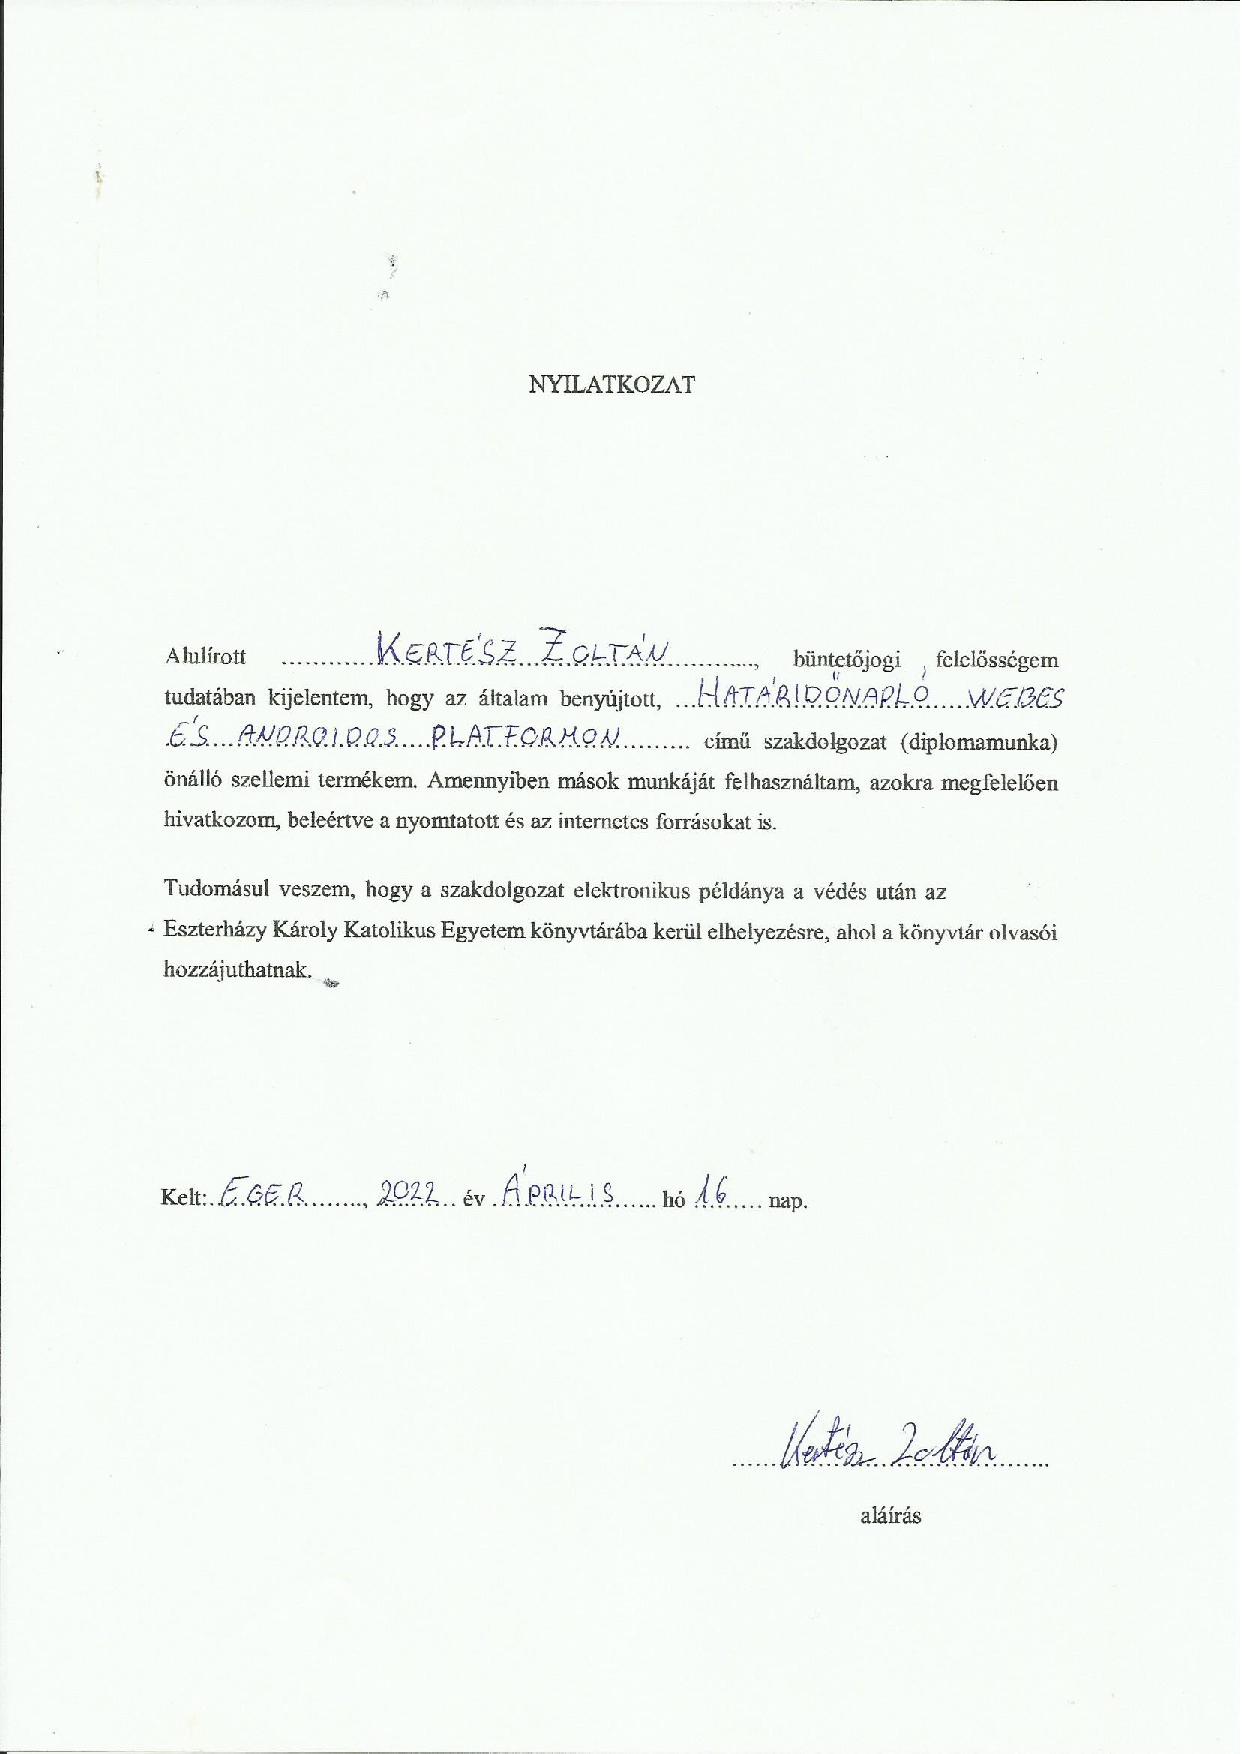
\includepdf[pagecommand={\thispagestyle{empty}}]{nyilatkozat.pdf}
\end{document}